\documentclass[10pt, t]{beamer}
% \usepackage[UTF8]{ctex}
\usepackage{amsmath}
\usepackage{setspace}
\usepackage{float} 
\usepackage{multido}
\usepackage{multirow}
\usepackage{array}
\usepackage{enumerate}
\usepackage{booktabs}
\usepackage{indentfirst} 
\usepackage[style=mla]{biblatex}
\usepackage{setspace}
\usepackage{subcaption}
\usepackage{hyperref}
\usepackage{textpos}

\makeatletter
\let\@@magyar@captionfix\relax
\makeatother

\definecolor{bladerunnerblue}{RGB}{41, 159, 163}
\definecolor{bladerunnerred}{RGB}{194,84,97}
\definecolor{themecolor}{RGB}{25,25,112} 
\definecolor{weak}{RGB}{150,150,150}

\renewcommand{\emph}[1]{{\color{bladerunnerblue}\textsl{#1}}}
\newcommand{\alarm}[1]{{\color{bladerunnerred}{#1}}}
\newcommand{\N}{\mathbb{N}}
\newcommand{\R}{\mathbb{R}}
\newcommand{\myseries}[2]{$#1_1,#1_2,\dots,#1_#2$}
\newcommand{\nullspace}{~\\[15pt]}
\newcommand{\remark}{\textbf{Remark: }}
\newcommand{\scp}[2]{\langle\,#1\,,\,#2\,\rangle} \newcommand{\scpp}{\langle\,\cdot\,,\,\cdot\,\rangle}
\newcommand{\weaken}[1]{{\color{weak}\textit{#1}}}
\newcommand{\underover}[3]{\underset{#2}{\overset{#3}{#1}}}
\renewcommand{\emptyset}{\varnothing}


\usetheme{Madrid}
\setbeamertemplate{navigation symbols}{}

\addtobeamertemplate{frametitle}{}{
\begin{textblock*}{100mm}(0.85\textwidth,-1cm)
\includegraphics[height=1cm]{../../logo.png}
\end{textblock*}}


\usecolortheme[named=themecolor]{structure}

\setbeamertemplate{items}[default]

\hypersetup{
    colorlinks=true,
    linkcolor=themecolor,
    filecolor=themecolor,      
    urlcolor=themecolor,
    citecolor=themecolor,
}

\title{VV186: Honors Mathematics}
\subtitle{\large Math Foundations}
\institute[UM-SJTU JI]{Univerity of Michigan-Shanghai Jiao Tong University Joint Institute}
\author{Xingjian Zhang}

\begin{document}

\begin{frame}
    \titlepage
    \begin{center}
        \includegraphics[height=2cm]{../../logo2.png}
    \end{center}
\end{frame}

\section{Introduction \& Tips}
\begin{frame}
    \frametitle{Outline}
    \begin{spacing}{1}
        \tableofcontents
    \end{spacing}
\end{frame}

\subsection{Introduction}
\begin{frame}
    \frametitle{Introduction}
    \begin{itemize}
        \item Xingjian Zhang
        \item Junior Student
        \item Major in ECE (JI) \& DS (UMich)
        \item VV285 TA in SU2020
        \item Key words:
              \begin{enumerate}
                  \item Conceptual Understanding
                  \item Interdisciplinary Spirits
                  \item Motivation and Essence
              \end{enumerate}
    \end{itemize}
\end{frame}


\subsection{Question Everything}
\begin{frame}
    \frametitle{Pay attention to...}
    Several things I want you to pay attention to:
    \begin{enumerate}
        \item \alarm{Be interactive.} Feel free to interrupt me at any time if you want to ask something or simply make some comments. You are free to discuss with your friend if you want, as long as your discussion is related to the course contents and your voice won't effect other students.
        \item Speak everything in \alarm{English} during the RC. This might be hard at the beginning, but you will soon get used to that.
        \item \alarm{``Question everything.''} Do not pretend to have understood everything. Maths is about strictness, abstraction and generalization. Understanding every basic concept is essential in our course. I will be quite ``push'' on checking your conceptual understanding. This process will be \textbf{annoying, tedious, but rewarding}. So Get prepared.
    \end{enumerate}
\end{frame}

\subsection{Recitation Class}
\begin{frame}
    \frametitle{Recitation Class}
    Each RC will contain some of these four parts:
    \begin{itemize}
        \item Recap of lecture
        \item Exercise
        \item Sample solutions to assignment problems
        \item Extension of lecture \\(marked with ``*''. e.g. ``* Propositional Logic and Predicate Logic'')
    \end{itemize}
    Apart from regular RC, \emph{big RC} will be held days before mid/final in order to help you prepare the exam better. \nullspace
    RC is \textbf{optional}. i.e. You are free to attend none of the RC if you think it is not helpful to you. Generally speaking, I will choose exercise whose difficulty is appropriate for most students. Thus, my RC might not be the right place for you if you want to seek for extremely difficult, exciting and interesting math problems. \nullspace
    I am personally excited in interdisciplinary thinking. So I will also try to give some examples in other math-related subjects. e.g. mechanics, electromagnetics, circuits, computer/data science and etc.
\end{frame}


\subsection{Notation}
\begin{frame}
    \frametitle{Notation}
    A \emph{notation} is a system of graphics or symbols, characters and abbreviated expressions, used (for example) in scientific disciplines to represent technical facts and quantities by convention.
    \nullspace
    Please follow Professor's notations. Keeping consistent in using notations is important because it helps you obtain a clear mind when we have a lot of complex concepts. Additionally, it makes your work more readable (for both your teammates and TAs).
    \nullspace
    Deduction will be given in assignment/exam if there is abuse/misuse of notations.
\end{frame}

\section{Logic, Set Theory, and Natural Numbers}
\subsection{Logic}
\begin{frame}
    \frametitle{Logic Foundation}
    Test your conceptual understanding:
    \begin{enumerate}
        \item statement
        \item negation
        \item conjunction, disjunction
        \item implication, equivalence
        \item tautology, contradiction
        \item contraposition (contrapositive)
        \item logically equivalent
    \end{enumerate}
    Ask yourself:
    \begin{itemize}
        \item How are they \textbf{defined}?
        \item What are they essentially? (2,3,4)
        \item What are their notations, if any?
        \item What is the difference between ``equivalence'' and ``logically equivalent''?
    \end{itemize}
    \textbf{Remark:} In reality, however, we will sometimes live with the ambiguity of equivalence and logically equivalent. 
\end{frame}

\begin{frame}
    \frametitle{Logical Quantifiers}
    Test your conceptual understanding:
    \begin{enumerate}
        \item universal quantifier
        \item existential quantifier
        \item vacuously true
    \end{enumerate}
    Ask yourself:
    \begin{itemize}
        \item How are they defined?
        \item What are their notations?
    \end{itemize}
\end{frame}

\begin{frame}
    \frametitle{* Propositional Logic and Predicate Logic}
    \begin{quote}

        \emph{Propositional logic} is the study of propositions, where a proposition is a statement that is either true or false. Propositional logic may be used to encode simple arguments that are expressed in natural language, and to determine their validity. The validity of an argument may be determined from truth tables, or using inference rules such as modus ponens to establish the conclusion via deductive steps. \emph{Predicate logic} allows complex facts about the world to be represented, and new facts may be determined via deductive reasoning. Predicate calculus includes predicates, variables and quantifiers, and a predicate is a characteristic or property that the subject of a statement can have.\footnote[frame]{
            \href{https://link.springer.com/chapter/10.1007/978-3-319-64021-1_6}{Propositional and Predicate Logic - Gerard O’Regan}
        }
    \end{quote}

    Without quantifiers, we could only define the propositional logic. This topic will be discussed in details in \textit{VE203: Discrete Mathematics}. Here, we only need a basic background knowledge of logics.
\end{frame}

\begin{frame}
    \frametitle{Exercise}
    Two simple exercises:
    \begin{enumerate}
        \item Let $A,B,C$ be statements. Use truth table to prove that $$(A\vee B )\wedge C \equiv (A\wedge C)\vee (B\wedge C).$$
        \item Interpret the following definition using English: \\[8pt] The real or complex sequence $\left(a_{n}\right): \Omega \rightarrow X, \Omega \subset \mathbb{N}$, $X=\mathbb{R}$ or $\mathbb{C},$ is said to \emph{converge} with limit $a \in X$ if
              $$
                  \underset{\varepsilon>0}{\forall}\quad \underset{N \in \mathbb{N}}{\exists}\quad \underset{n>N}{\forall}\quad\left|a_{n}-a\right|<\varepsilon
              $$
              Find the negation of above predicate. \weaken{(If its negation is true, we say that the sequence is not convergent with $a$.)}
    \end{enumerate}
\end{frame}

\subsection{Set Theory}
\begin{frame}
    \frametitle{Set Foundation}
    Test your conceptual understanding:
    \begin{enumerate}
        \item set
        \item empty set
        \item (proper) subset
        \item power set
        \item cardinality
    \end{enumerate}
    Ask yourself:
    \begin{itemize}
        \item How are they defined?
        \item How to prove two sets $A, B$ are equal? (at least two ways)
        \item Why empty set $\emptyset$ is a subset of any set?
    \end{itemize}
    \pause
    \textbf{Remark:} The sets are defined through predicates. Correspondingly, the operations on sets are defined through operations on predicates.
\end{frame}

\begin{frame}
    \frametitle{Set Operation}

    The \emph{union}, \emph{intersection}, and \emph{difference} of sets is defined by
    $$\begin{array}{l}
            A \cup B:=\left\{x: P_{1}(x) \vee P_{2}(x)\right\}   \\
            A \cap B:=\left\{x: P_{1}(x) \wedge P_{2}(x)\right\} \\
            A \backslash B:=\left\{x: P_{1}(x) \wedge\left(\neg P_{2}(x)\right)\right\}
        \end{array}$$
    We can then further define the \emph{complement} and \emph{disjoint}.
    \nullspace
    \textbf{Remark:} From the definition above, we can find an analogy between set operation and logic operation. See the following exercise.
\end{frame}

\begin{frame}
    \frametitle{Exercise}
    Prove
    $$(A\cup B)\cap C = (A\cap C)\cup (B\cap C)$$
    $$(A\cup B)\backslash C = (A\backslash C)\cup (B\backslash C)$$
    in two ways:
    \begin{itemize}
        \item by definition
        \item by ``subset''
    \end{itemize}
\end{frame}

\begin{frame}
    \frametitle{Other Notation about Set Operations}
    $$\begin{array}{l}
            \underover{\bigcup}{k=0}{n} A_{k}:=A_{0} \cup A_{1} \cup A_{2} \cup \cdots \cup A_{n} \\
            \underover{\bigcap}{k=0}{n} A_{k}:=A_{0} \cap A_{1} \cap A_{2} \cap \cdots \cap A_{n}
        \end{array}$$
    How to properly generalize the notation to $n=\infty$?
\end{frame}

\begin{frame}
    \frametitle{Ordered Pairs}
    A set does not contain the information about the order of its elements.  However,
    sometimes it is convenient or necessary to have such an ordering. This is
    achieved by defining an \emph{ordered pair}, denoted by
    $$(a,b)$$

    If $A, B$ are sets and $a \in A, b \in B,$ then we denote the set of all ordered pairs by
    $$
        A \times B:=\{(a, b): a \in A, b \in B\}
    $$
    $A \times B$ is called the \emph{cartesian product} of $A$ and $B$. we may abbreviate cartesian product
    using exponents. (What does an element in $\R^3$ represents?)
    \nullspace
    \textbf{Remark:} * Using ordered pairs, one can then define \emph{ordered triples} and, more
    generally, \emph{ordered n-tuples}. For elements $x_0 ,...,x_n$ , define
    $$(x_0 ,...,x_n ) = (x_0 ,(x_1 ,...,x_n ))$$
    This is an example of a \emph{recursive definition}. Correspondingly, one can define the \emph{n-fold cartesian product} of sets. 
\end{frame}

\begin{frame}[allowframebreaks]
    \frametitle{Some Insight}

    \textbf{Remark:} * Moreover, the natural numbers can be constructed rigorously from set theory using empty set $\emptyset$ and successor operation $S(x)=x\cup \{x\}$. In \textit{Zermelo–Fraenkel (ZF) set theory}, the natural numbers are defined recursively like this:
    $$\begin{array}{l}
        0:=\emptyset \\
        1:=S(\emptyset)=\{\emptyset\} \\
        2:=S(S(\emptyset))=\{\emptyset,\{\emptyset\}\}
        \end{array}$$
    Then we use set $\N_{def }$ to interprets the natural numbers where
    $$\mathbb{N}_{def}=\{\emptyset,\{\emptyset\},\{\emptyset,\{\emptyset\}\}, \ldots\}$$
    The above is just a brief introduction of what have been mentioned in the lecture. Do not worry if you cannot get the points because it will be discussed in details in VE203.
    \newpage
    \begin{quote}
        The result comes from a strong historical desire to find a list of axioms from which all mathematical truths could be proved in a first-order system. With the advent of calculus, people began to prove all types of completely incorrect statements by their cavalier manipulation of the infinite. This fact, coupled with the discovery of Russell's Paradox, led to people to believe that there should be a more systematic way of theorem-proving. It was later proved impossible by Godel to find such a comprehensive system, even if infinitely many axioms were allowed. Still, most results of interest can be proved from the set-theoretic construction of mathematics known as ZFC set theory. One of the axioms is the existence of the natural numbers. \textbf{It is generally accepted that one should take as few axioms as possible. Also, it actually turns out proof-wise to be easier to construct the integers than assuming their existence, as it would be more difficult to define the addition and multiplication operations on them.} These are the two largest reasons why. We actually construct the natural numbers in a sense as well.\footnote[frame]{\href{https://math.stackexchange.com/questions/2537487/what-is-the-benefit-in-constructing-the-integers-from-natural-numbers}{Why we construct natural numbers by set theory? - math.stackexchange}}
    \end{quote}
    \newpage
    The order of introduction to various concepts in vv186-vv285-vv286 is not arranged in a way that from easy to hard, simple to complex. Instead, the first priority is always \textbf{strictness}. So it is a very common situation where we use a quite complex structure to represent some seemingly naive concepts. This might not be intuitive, but it is going to be useful and rigorous.
    \nullspace
    Some examples:
    \begin{itemize}
        \item Ordered pairs
        \item Natural numbers
        \item Exponential functions
        \item Triangular functions
        \item Matrices
        \item ...
    \end{itemize}
\end{frame}

% \begin{frame}
%     \frametitle{Russel Antinomy}
%     Naive set theory allows the unrestricted formation of sets. In particular, \textbf{Unrestricted
%     self-reference} has long been known to be problematic. This was eventually elaborated by Russel. In brief, 
%     \begin{center}
%         The predicate $P(x): x \notin x$ does not define a set $A=\{x: P(x)\}$.
%     \end{center}
%     (How did we prove this?)
% \end{frame}

% \subsection{Natural Number and Mathematical Induction}
% \begin{frame}
%     \frametitle{Natural Number}
%     What is the seven properties of natural numbers' operations?\nullspace
%     \pause 
%     \begin{enumerate}
%         \item 
%         associativity$\times 2$
%         \item
%         existence of neutral element$\times 2$
%         \item commutativity$\times 2$
%         \item distributivity. 
%     \end{enumerate}
% \end{frame}

% \begin{frame}
%     \frametitle{Notation for Addition \& Multiplication}
%     \begin{figure}[H]
%     \centering
%     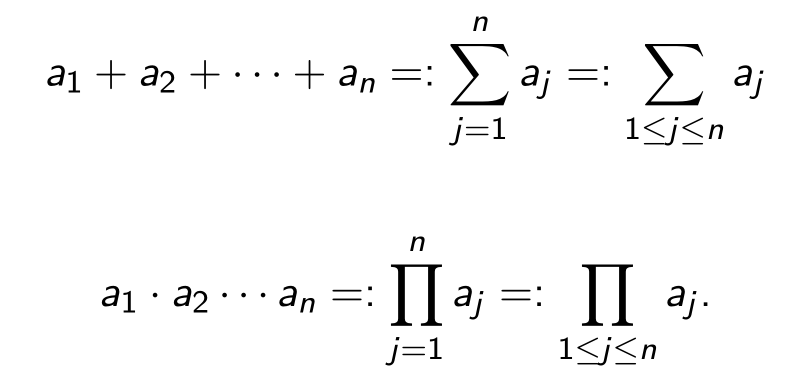
\includegraphics[width=0.5\textwidth]{2020-09-23-13-08-15.png}
%     \end{figure}
    
    

% \end{frame}

% \begin{frame}
%     \frametitle{Mathematical Induction}

%     \begin{figure}[H]
%     \centering
%     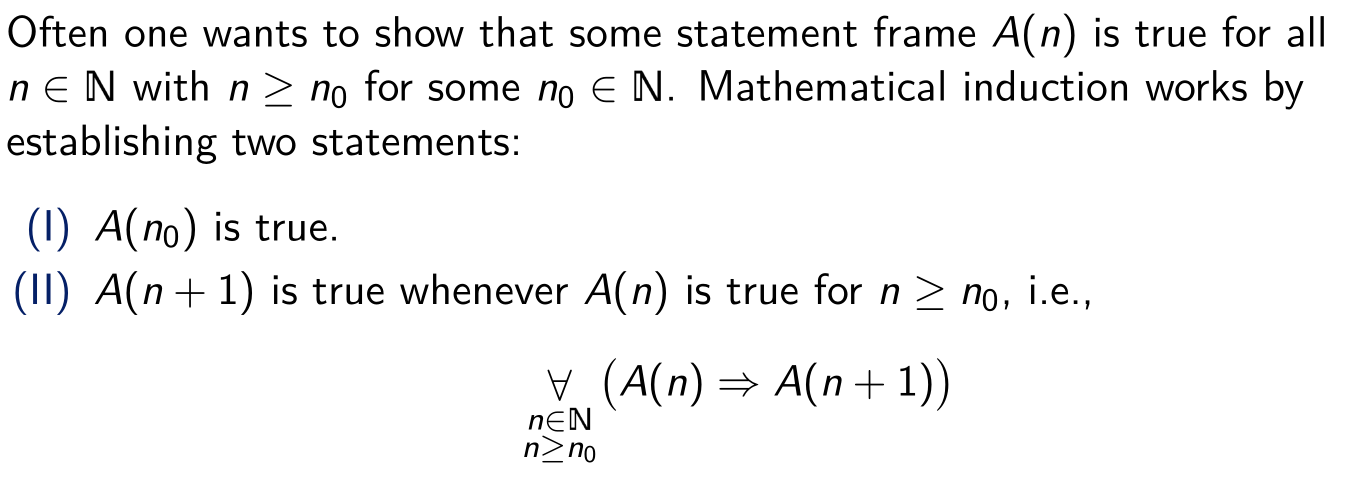
\includegraphics[width=0.9\textwidth]{2020-09-23-12-37-23.png}
%     \end{figure}
%     Straightforward Exercise:\nullspace Prove 
%     \begin{center}
%         For all $n\in \N$, $5^n - 1$ is divisible by 4.
%     \end{center}
% \end{frame}

% \begin{frame}[allowframebreaks]
%     \frametitle{Conceptually Interesting Exercise}

%     Let's see an interesting problem. What is going wrong in the proof?
%     \begin{figure}[H]
%     \centering
%     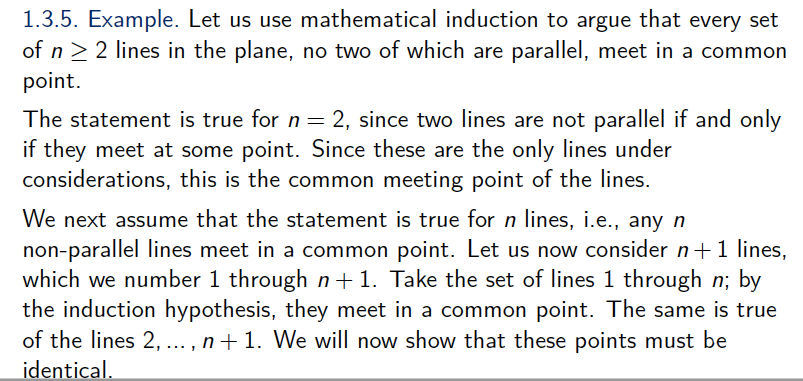
\includegraphics[width=0.9\textwidth]{2020-09-23-13-12-35.png}
%     \end{figure}
%     \begin{figure}[H]
%     \centering
%     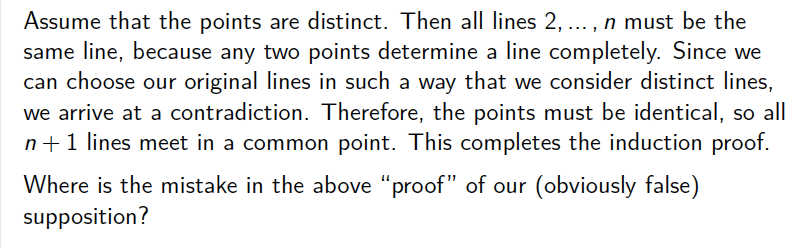
\includegraphics[width=0.9\textwidth]{2020-09-23-13-13-41.png}
%     \end{figure}
%     \textbf{Hint:} Start by considering the case where $n=3$, find some contradiction to invalidate the above proof.\nullspace
%     \textbf{Remark:} Induction can sometimes be tricky. Before using it, examine the complex level of the problem, because using induction is sometimes
%     much more complicated than using a ``direct'' method to prove a statement.
% \end{frame}

\begin{frame}
    \frametitle{Tips on Assignments}
    \begin{itemize}
        \item Please read the introduction on P.1 of Assignment 1 carefully.
        \item Discuss with your teammates. If you haven't figure out a solution, learn from your teammate. If you know how to do it, share your ideas with your teammates. Both will help you learn better. (The later way helps you consolidate your knowledge. See \href{https://medium.com/taking-note/learning-from-the-feynman-technique-5373014ad230}{Learning From the Feynman Technique})
        \item The knowledge we learn in the first two weeks are very fundamental. And the real interesting part (\textit{Real Functions, Convergence and Continuity}) is just coming up!
    \end{itemize}
\end{frame}

\begin{frame}
    \frametitle{End}
    \vspace{2.2cm}
    \begin{center}
        \Large
        Have Fun \\
        And \\
        Learn Well!\footnote[frame]{Special acknowledgement to former TA Zhang Leyang, who offered many exercises and advice to my recitation class.}
    \end{center}
\end{frame}


\end{document}